The adjective \todef{recursive} means ``defined in terms of itself.''
As computer scientists, we frequently run into recursion in the form
of recursive functions, which are functions that call themselves
(directly, or indirectly through another function).
However, as we see below, another very important
application is recursive definitions of objects.
We will explore recursion through several examples.

\begin{figure}[htb]
\centering
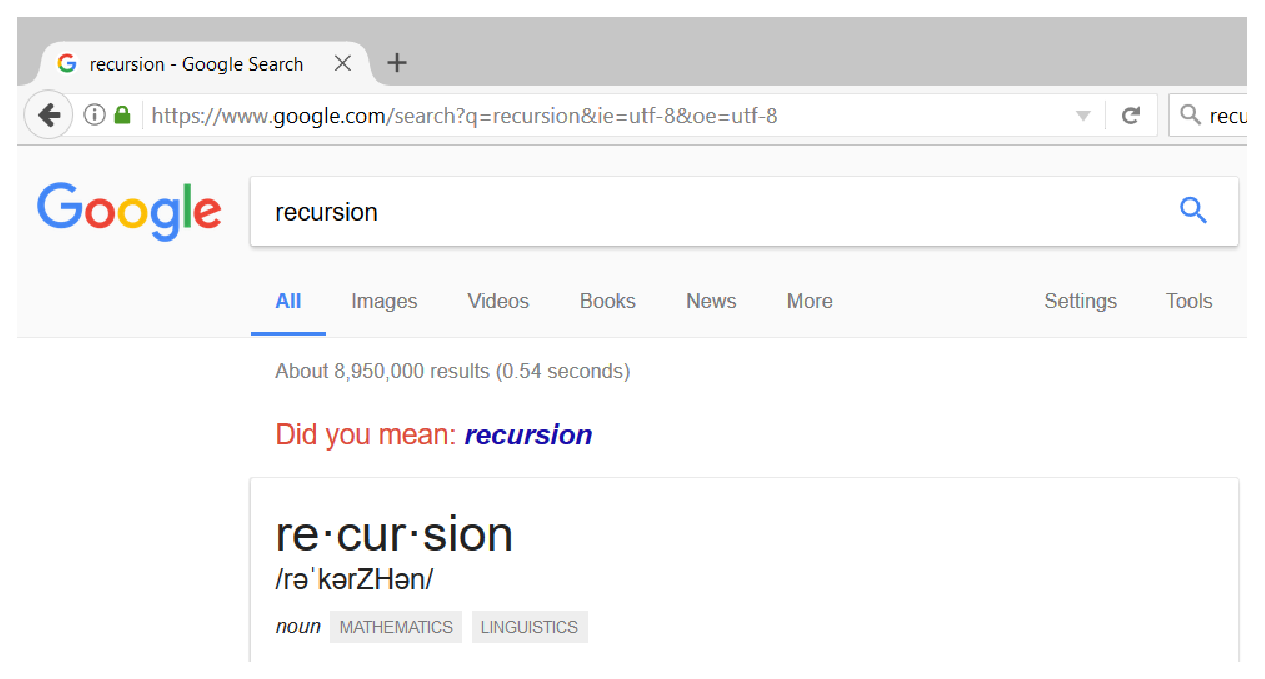
\includegraphics[scale=0.6]{comics/recursion-screenshot.eps}
\caption{What happens when you Google ``recursion''}
\end{figure}


\section{Computing Factorials}
Our first example, which you have likely seen before,
is to compute the factorial of $n$, which is defined 
as $n! = n \cdot (n-1) \cdot (n-2) \cdots 2 \cdot 1 = \prod_{i=1}^n i$.
Of course, we could use iteration (a simple \code{for} loop) to
compute $n!$.
\begin{verbatim}
int factorial(int n) {
    int p=1;
    for (int i=1; i<=n; i++)
        p*= i;
    return p;
}
\end{verbatim}

This is a perfectly valid, and probably even the best,
way to compute the factorial of a number.
However, in this section, we will use this very easy example
to illustrate how recursion works.

Looking at the definition, we observe that $0! = 1$ (by definition),
and $n! = n \cdot (n-1)!$.
This suggests a recursive solution for computing factorials:

\begin{verbatim}
int factorial (int n) {
    if (n==0) return 1;
    else return n*factorial(n-1);
}
\end{verbatim}

Notice that the function \code{factorial} calls itself;
this is what makes our implementation recursive.
Many students have trouble thinking about recursion initially.
Our instinct is often to make a complete plan for the computation:
first multiply $n$ with $n-1$, then with $n-2$, and so on,
all the way to $1$. 
In a recursive solution, we instead treat most of the work as a
``black box:'' we do not really worry \emph{how} the call with
parameter $n-1$ will obtain the correct results, and just trust
\emph{that} it does.
Of course, that only works if the function is actually correct,
but since you yourself are writing the function, you can make sure
that the outcome will be correct \emph{assuming} that what you got
from the recursive call was correct.

To illustrate this concept in even more detail, consider computing
$n!$ with a group of classmates.
Each student is in charge of computing the value $n!$ only for one
particular number $n$.
The student in charge of computing $5!$ relies on another student to
compute $4!$, then uses her result and multiplies it with 5.
So we get a long chain of work delegation,
where every student only carries out one multiplication
and relies on another student for all the preceding work.
The important insight here is that the student who must compute
$5!$ does \emph{not} need to know how the other student computes $4!$;
so long as the $4!$ student got the right result,
it can just be plugged in.
Maybe the $4!$ student used a loop instead of recursion?
Or maybe she is just really good at guessing factorials.
It does not matter to the $5!$ student --- so long as the result is
right, he can use it.

To recap this once more, in a recursive solution,
we do not have to think of every step,
nor do we have to keep track of various intermediate results,
as those are returned as values by the other function calls. 
Students getting started on recursion often try as hard as possible to
have recursion emulate loops, by passing around ``global variables''
(or pointers to variables, which amounts to the same thing)
that are altered and store intermediate results.

This type of thinking can take a while to get used to,
but once you firmly grasp it, a lot of things
--- most importantly induction and, later on, dynamic programming ---
will come to you much more easily.

Two things that pretty much all correct recursive functions share are
the following:

\begin{itemize}
\item A recursive function needs one or more base case: at some point,
  the function must hit a point where it will no longer call itself
  (like the \code{n==0} case for the factorial). 
  Otherwise, the function will keep calling itself forever, and
  eventually run out of stack memory.
\item Recursive calls must have ``smaller'' inputs than the main
  input. In the case of the \code{factorial} function, the recursive
  call within \code{factorial(n)} was for \code{factorial(n-1)}.
  In this case, it is clear that $n-1$ is ``smaller'' than $n$.
  In other cases, ``smaller'' refers to the remaining size of an
  array, or even a number that is closer to an upper bound.
  (For instance, the base case could be \code{i==n}, and the call with
  input $i$ could be to $i+1$.)
\end{itemize}

Let us look quickly at two examples violating these conditions, and
see what happens.

\begin{verbatim}
int UCLAfact (int n) // apologies to our neighboring school
{
   if (n == 0) return 1;
   else return UCLAfact (n); // error: input not getting smaller!
}

int NDfact (int n)
{
   return n*NDfact (n-1); // ...this doesn't stop!
}
\end{verbatim}

Neither of these functions will terminate.
In the first example, we do have a base case, but the recursive call
has the same size.
It is of course correct that $n! = n!$
(which is what the function uses),
but it doesn't help us compute it.
In the second example,
we do have a smaller input in the recursive call,
but no base case, so the function will continue calling itself
with different values forever
(or until it runs out of stack space and crashes).

\begin{figure}[htb]
\centering
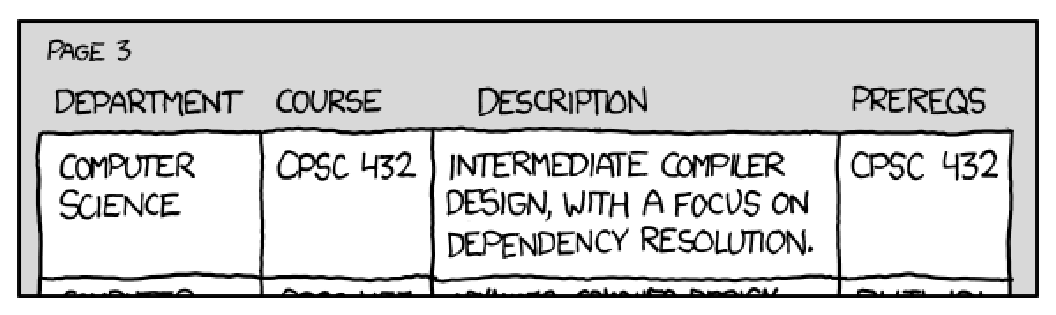
\includegraphics[scale=0.6]{comics/xkcd_dependencies.eps}
\caption{XKCD \# 754: Recursive Course Dependencies}
\end{figure}

\section{Binary Search}
Admittedly, computing factorials is not a very strong example to show
why recursion is useful, since the iterative solution is short and
elegant. However, we were able to illustrate some of the important
properties of recursion with an easy enough general setup.
Next, let us look at a somewhat more challenging task:
Given a (pre-sorted) array of integers in increasing order, find the
location of a target element, or return -1 if it is not in the array.
(If instead of integers, our array contained the names of students in
the class, we would have the setting we looked at in
Example~\ref{exm:overview:binary-search}.)

This task is accomplished using the \todef{Binary Search} algorithm:
Check the middle of the remaining array.
If the element is there, we are done.
If the desired element is smaller,
continue searching to the left of the middle element;
otherwise, continue searching to the right.
A corresponding iterative solution looks as follows:

\begin{verbatim}
int binarySearch (int n, int* b, int len) 
{
   int lo = 0, hi = len, mid;
   while(lo <= hi) {
       mid = (hi+lo)/2;
       if (b[mid]==n) return mid;
       else if(n < b[mid])
                 hi = mid-1;
            else lo = mid+1;
    }
    return -1;
}
\end{verbatim}

A recursive solution looks as follows:

\begin{verbatim}
int recSearch(int n, int* b, int lo, int hi) {
    if (hi < lo) return -1;  // not in the array
    else 
      {
        int mid = (hi+lo)/2;    // the midpoint of the array
        if (n == b[mid]) return mid;    // we found it
        else if (n < b[mid]) 
             return recSearch(n, b, lo, mid-1);  // element to the left of the midpoint
        else return recSearch(n, b, mid+1, hi);  // element to the right of the midpoint
      }
}
\end{verbatim}

To start the search, we call the function as \code{recSearch(n, b, 0, len)}.
Whether you like the iterative or the recursive solution better here
may be a matter of taste, but notice that there is a certain elegance
to the recursive solution.
When we have decided where the element must be (to the left or the right),
rather than updating a variable and repeating,
we simply ask the function to find it for us in that (correct) subarray,
and return its return value unchanged.
This is akin to delegating the task of finding the number in the
smaller array to another student, as we discussed earlier.

Notice that both implementations will work whether the array has an
even or odd number of elements.
If we hadn't written \code{mid-1} and \code{mid+1} for the recursive calls,
we might have needed another base case when \code{lo == hi}. 

Let us check that we satisfy the two conditions above for a recursive
solution to have a chance to work:
\begin{itemize}
\item If the array is empty (which is the case \code{hi < lo}),
  the function returns directly,
  reporting that the element was not found. 
\item If \code{n} is less than the midpoint,
  the function recurses on the left half of the array;
  otherwise, on the right half.
  In either case, because we eliminate at least the midpoint,
  the remaining array size is strictly smaller than before.
\end{itemize}

One of the things that can be confusing about recursion is that there
seem to be many ``active'' versions of the function at once.
What is ``the'' value of variables like \code{n}, \code{lo},
\code{hi}, or \code{mid}?
After all, different invocations of the function will have different
values for them.
To solve this ``conundrum,'' remember from our overview of memory that
local variables are stored on the stack, and translated into memory
locations by the compiler and OS.
Thus, when the function \code{recSearch(12,b,0,10)} calls
\code{recSearch(12,b,0,4)}, their variables \code{lo}, \code{hi}
translate to completely different memory locations.
When the call \code{recSearch(12,b,0,4)} executes,
the values are \code{lo=0, hi=4}, and \code{mid=2} will be computed.
In the call \code{recSearch(12,b,0,4)},
we instead have \code{lo=0, hi=10, mid=5}.
The computer has no problem with the same variable name,
as only one meaning of the variable is in scope at a time.

\section{Enumerating all Binary Strings of a given length}
The first two examples we saw were pretty easily coded with a simple loop.
In general, if you have a recursive function that uses just one
recursive call to itself, it is often easily replaced by a loop.
Recursion becomes much more powerful
(as in: it lets you write short and elegant code for problems that
would be much more messy to solve without recursion)
when the function calls itself multiple times.

We will see several examples of that later in class with some clever
recursive sorting algorithms and other algorithms.
Another very common application is \todef{exhaustive search},
which is frequently based on enumerating all binary strings or strings
over some other set of letters (called ``alphabet'').
In turn, such an enumeration forms the basis of a technique called
``Backtracking.''

To derive a recursive solution for this problem,
let us return to our earlier thought experiment of students delegating
subtasks to each other.
Suppose that you have been asked to print all binary strings of length
3, but you can call on classmates who have expertise in printing
binary strings of length 2.
And you are lazy, so you would like to utilize this expertise to the
maximum.
Take a quick look at Table~\ref{tab:recursion:binary}.
It shows all binary strings of length 3,
arranged in a suggestive pattern.
Looking at the top part,
we see the digit `0' always in the first position, 
and followed by all binary strings of length 2.
Then, in the bottom part, we have the digit `1' in the first position,
followed again by all binary strings of length 2.

\begin{table}[htb]
\begin{tabular}{|c|c c|}
  \hline
  0 & 0 & 0 \\
  0 & 0 & 1 \\
  0 & 1 & 0 \\
  0 & 1 & 1 \\ \hline

  1 & 0 & 0 \\
  1 & 0 & 1 \\
  1 & 1 & 0 \\
  1 & 1 & 1 \\ \hline
\end{tabular}
\caption{The eight binary strings of length three. \label{tab:recursion:binary}}
\end{table}

So if you want to save yourself a lot of work, you could write `0' in
the first position, and then ask your classmate to fill in all the
strings of length 2 in the remaining positions
(and print the whole thing).
Then, when your classmate is done, you can overwrite your `0' with a
`1', and then ask the same classmate to repeat what he did earlier.

Of course, there was nothing specific about the numbers 3 and 2 here;
you could do the same thing for 42 and 41
(except we couldn't fit the example table in these notes).

Using the ideas we just worked out, we can now write down a recursive
algorithm.

\begin{verbatim}
void binaryStrings (int length, string s, int pos)
{
   if (pos == length) cout << s << endl;
   else
      {
        s [pos] = '0';
        binaryStrings (length, s, pos+1);
        s [pos] = '1';
        binaryStrings (length, s, pos+1);
      }
}
\end{verbatim}

In this piece of code, \code{length} is the length of the binary
strings you are trying to print,
\code{s} is the string you are building (with your classmates),
and \code{pos} is the position you personally are in charge of.
As we said above, you do your part by putting `0' in your position,
then delegating the rest of the task to your classmate in charge of
position \code{pos+1}.
Then, you put `1' in your position, and again delegate the rest to
your classmate in charge of position \code{pos+1}.
Notice a few things here:
\begin{itemize}
  \item The first call would be \code{binaryStrings (0, s, length)},
    where \code{s} is some string that we allocated to be of the given
    length.
  \item We chose our base case to be that \code{pos==length}, not
    \code{pos==0}.
    We could have done that, too (or maybe \code{pos==-1}),
    in which case we would need to replace \code{pos+1} with
    \code{pos-1} in the recursive calls.
  \item The ``size'' of the input to solve is measured as
    \code{length-pos} here; whenever a call happens with \code{pos+1},
    this size (how many more digits need to be filled in) gets
    smaller, and the program gets ``closer'' to the base case.
  \item There was nothing particularly special about the strings being
    binary. Enumerating numbers in any base, or printing strings over
    any alphabet, is an easy modification of the above code.
    (Hint: \code{for} loops might come in handy.)
\end{itemize}

Experience tells us that such code is often difficult for students to
understand at first.
We recommend going through it by hand for \code{length==3} and
\code{length==4} and keeping track of all recursive function calls and
their variables and where they are in their execution.

\section{The $n$-Queens problem (*)}
In the $n$-queens problem, you want to place $n$ queens on an 
$n \times n$ chessboard (square grid). 
Each queen occupies one square on a grid and no two queens share the
same square. Two queens are \emph{attacking} each other if one of
them can travel horizontally, vertically, or diagonally and hit the
square the other queen is on.
The problem is to place the queens such that no two queens are
attacking each other.
For instance, what you see in Figure~\ref{fig:queens} is not a legal
solution: the queens in columns 1 and 3 attack each other diagonally,
as do the the queens in columns 2 and 3.
(All other pairs of queens are safe, though.)

\begin{figure}[htb]
\begin{center}
\setlength{\unitlength}{1cm}
\begin{picture}(5,5)
\linethickness{0.02mm}
\multiput(0,0)(0,1){6}{\line(1,0){5}}
\multiput(0,0)(1,0){6}{\line(0,1){5}}
\large
\put(0.4,0.4){Q}
\put(4.4,1.4){Q}
\put(2.4,2.4){Q}
\put(1.4,3.4){Q}
\put(3.4,4.4){Q}
\end{picture}
\caption{Illustration of the 5-queens problem \label{fig:queens}}
\end{center}
\end{figure}

Before we try to solve the problem, we make some observations.
Because queens attack each other when they are in the same row or
column of the chessboard, we can phrase the problem equivalently as
follows: place exactly one queen per row of the board such that no two
queens are in the same column or attack each other diagonally.

Thus, each row has a designated queen, and for each queen,
the program needs to try all possible columns.
If we didn't also need to check the diagonals,
this would look very similar to the binary strings enumeration we just
saw.
Each of the $n$ rows is like a position in the binary string,
and the column of its designated queen is like the character we chose,
ranging also from $0$ to $n-1$.
To avoid having to pass around variables like \code{s} and
\code{length} in \code{binaryStrings}, we will assume that we have
global variables

\begin{verbatim}
int *q; // array for the positions of the queens
int n;  // size of the grid
\end{verbatim}

Adapting our earlier \code{binaryStrings} code, the basic scaffold of
our $n$-queens solution will look as follows:

\begin{verbatim}
void queenSearch (int row)
{
   if (row == n) printSolution (); // that function shows the layout
   else
      {
        for (q[row] = 0; q[row] < n; q[row]++)
           {
               queenSearch (row+1);
           }
      }
}
\end{verbatim}

This short piece of recursive code will try all combinations of
positions for the $n$ queens, for a total of $n^n$ ways of placing
the $n$ queens. 
However, so far, it prints everything, including illegal solutions;
we have to modify the code to not print solutions if two queens can
attack each other.
There are a few ways to do this, but perhaps the most intuitive is to
keep an array of size $n \times n$ of positions that are currently
threatened by one or more queen.
That way, we can avoid placing a queen in a threatened position in the
first place, which should be much faster than only checking at the
very end.
Doing this kind of early checking is often called ``Backtracking.''

To decide on what we need to store in the array, we can think ahead a
bit about how we will update the array.
When we place a new queen, we will need to mark everything it
attacks as ``threatened.''
Then, when we remove the queen later to try a different position,
we want to mark those positions as ``not threatened.''
But we have to be careful: if a position is threatened by two queens,
and we remove the second threat, the position is still threatened, so
we cannot mark it ``not threatened.''
So it turns out to be better to mark \emph{how many} currently placed
queens threaten each position.

This suggests that we want a 2-dimensional array of \code{int}.
We will call that array \code{int **t} (for ``threatened''),
and also make it a global variable.
Because it is a two-dimensional array, it needs to be a pointer to a
pointer, and we have to be careful to initialize it fully and allocate
the memory for it dynamically.
Using our new array \code{t} (which we need to initialize to all-0
outside the \code{queenSearch} function), the new version of
the recursive function looks as follows:

\begin{verbatim}
void queenSearch (int row)
{
   if (row == n) printSolution (); // that function shows the layout
   else
      {
        for (q[row] = 0; q[row] < n; q[row]++)
           if (t[row][q[row]] == 0)
           {
               addToThreats (row, q[row], 1);
               queenSearch (row+1);
               addToThreats (row, q[row], -1);
           }
      }
}
\end{verbatim}

The new code \code{if (t[row][q[row]] == 0)} only places a queen if
the current candidate column is not threatened.
Then, it adds one threat to all positions threatened by the queen we
just placed.
After the recursive call returns, the queen gets removed (and placed
somewhere else), so we subtract one threat from all positions it
reaches; hence the -1.
Notice that this code is very compact, and not too big of a deviation
from what we saw for enumerating all binary strings.
This elegance is frequently a feature of recursive Backtracking
solutions.

Now, basically all that remains is to write the function \code{addToThreats},
which increases the number of threats for the threatened squares.
The function should mark all places on the same column, and on the two
diagonals below the current square.
For the latter, we need to make sure not to leave the actual grid.
Looking at it a little carefully,
you will see that the following function does that:

\begin{verbatim}
void addToThreats (int row, int column, int change)
{
   for (int j = row+1; j < n; j++)
      {
         t[j][column] += change;
         if (column+(j-row) < n) t[j][column+(j-row)] += change;
         if (column-(j-row) >= 0) t[j][column-(j-row)] += change;
      }
}
\end{verbatim}

Finally, we need to write our \code{main} function that reads the
size, creates the dynamic arrays, initializes them, and starts the
search.

\begin{verbatim}
int main (void)
{
   cin >> n;
   q = new int [n];
   t = new int* [n];
   for (int i = 0; i < n; i++)
      {
        t[i] = new int [n];
        for (int j = 0; j < n; j ++)
            t[i][j] = 0;
      }
   search (0);
   delete [] q;
   for (int i = 0; i < n; i ++) delete [] t[i];
   delete [] t;
   return 0;
}
\end{verbatim}

If you do not yet fully understand how the above solution works, 
try tracing its execution by hand on a $5 \times 5$ board, by
simulating all the $q[i]$ variables by hand.
That will probably give you a good idea of Backtracking.

\section{Some General Comments on Recursive Functions}

At a high level, there are two types of recursion:
\todef[recursion]{direct} and \todef[recursion]{indirect}. 
Direct recursion happens when a function $f$ calls itself.
That is what we have seen so far.
Not quite as frequent, but still quite common, is \emph{indirect}
recursion: you have two functions $f,g$, and $f$ calls $g$, and $g$
calls $f$.
There is nothing particularly deep about this distinction:
we are mentioning it here mostly so that you are familiar with the
terms.
If you find yourself using indirect recursion and running into
compiler errors, the problem could be that one of the two function
definitions has to be first, and when you define that function,
the compiler does not know about the other function yet.
The way around that is as follows. (In the examples, we assume that our
functions are from \code{int} to \code{int}, but there is nothing
special about that.)

\begin{verbatim}
int f (int n); // just a declaration of the signature (this will often go in the .h file)

int g (int n)
{ 
  // insert code for g here, including calls to f
}

int f (int n)
{ 
  // insert code for f here, including calls to g
}
\end{verbatim}

This way, when the compiler gets to the definition of \code{g},
it already knows that there is a function \code{f};
when it gets to \code{f}, you have already defined \code{g}.

\medskip

For direct recursion, there are are two more common terms you
should know about: \todef[recursion]{head} recursion, and
\todef[recursion]{tail} recursion. 
These two terms apply when the recursive function only calls itself
once, and they refer to \emph{when} the recursive call happens.
If the recursive call happens at the \emph{end} of a function,
this is called tail recursion.
Tail recursion is particularly easily replaced by a loop.
When the recursive call happens earlier than the end (e.g., at the
beginning), this is called head recursion.
Head recursion turns out to be able to easily do some surprising
things, such as print strings or linked lists in reverse order.
The distinction is not really a huge deal,
but it is probably good to have heard the terms,
since such questions are often part of job or internship interviews.

\medskip

Another thing to keep in mind is that there are some programming
languages (called \todef{functional languages}) in which typically all
problems are solved using recursion.
Several of them do not even have loops.
Some examples of such languages are ML (or its variant OCAML),
Lisp, Scheme, Haskell, Gofer. There are others.
Some of these (in particular, ML) are actually used in industry,
and Lisp is used in the Emacs editor.

Functional languages make functions much more central than procedural
languages do.
It is very typical in functional languages to write a function that
takes another function as an argument\footnote{This can also be done
  in most other languages, but is typically rarely used.}.
A typical use is a function $g$ that operates on an array or list,
and gets passed another function $f$ as an argument;
it then applies $f$ to each element of the array/list. 
(For instance, you could have a function that turns each entry of an
array into a string.)
This operation is called \todef{map}.
Another common thing is to have a function $h$ that applies some other
function to compute a single output from an entire array/list.
An example would be to sum up all elements of an array/list,
or to compute the maximum.
This operation is called \todef{reduce}.

Programs that are written by applying only these two types of
operations can often be very easily parallelized over large
computation clusters, which is why the \todef{Map-Reduce} framework has
become quite popular lately (e.g., in Google's \todef{Hadoop}). 
It has led to a resurgence in interest in some aspects of functional
programming. 

From a practical perspective, when you write functional programs,
it often takes longer to get the program to compile,
because many logical mistakes that lead to weird behavior in C++ can't
even be properly implemented in a functional language.
Once a functional program compiles correctly,
it is much more often bug-free than a procedural program
(assuming both are written by fairly experienced programmers).

\section{Recursive Definitions} \label{sec:recursion:definitions}

So far, we have talked about recursion as a programming technique.
An almost equally important application of recursion is as a way of
specifying objects concisely, by virtue of recursive definitions.
These will come in very handy later on when we will use them to define
lists, stacks, heaps, trees, and others.
To be ready to use recursive definitions when we need them,
we will practice here with a few easier recursive definitions.
The first few of these recursive definitions are examples that you can
define pretty easily without recursion
(just like our earlier examples of using recursion
as a programming technique),
while the later ones may be more involved
(and would be very hard to define non-recursively).

\begin{enumerate}
\item A string of (lower-case) letters is either:
(1) the empty string (often written as $\epsilon$ or $\lambda$), or
(2) a letter `a'--`z', followed by a string of letters.

The recursion happens in case (2), and case (1) is the base case.
Of course, for this one, we could just have said that a string is a
sequence of 0 or more lower-case letters, which would have been just
fine.
But we are practicing recursion on easy examples here.

We should convince ourselves that this captures exactly strings,
and nothing else.
Can we get all strings? Sure!
If the string is not empty, then it must have a first character,
and a remainder of the string.
The remainder can be constructed (induction proof),
and by concatenating the first character to it, we get the whole string.
That the empty string can be built is our base case.
In return, we cannot build any non-strings this way: if you put one
more character at the beginning of an existing string, you still have
a string.

\item A non-negative integer is either:
(1) the number 0, or
(2) $n+1$, where $n$ is a non-negative integer.

Here, defining \emph{what exactly} integers are without referring to
integers in the first place may be a little puzzling.
Recursion helps with that.
It says that there is a first one (the number 0),
and a way to get from one to the next one.
In this sense, 4 is really just shorthand for $0+1+1+1+1$,
which is in fact what computer proof systems use.

Again, we should convince ourselves that this definition gives exactly
the non-negative integers, and nothing else.
First, 0 is a non-negative integer.
And if you have a non-negative integer and add 1,
you get another non-negative integer.
So we do not get anything that is not a non-negative integer.

In the other direction, we do get 0.
And if we are thinking about getting a number $n > 0$,
we can assume by induction that we get $n-1$.
Then, adding 1 gives us n.
So we get \emph{all} non-negative integers.

\item A palindrome is either:
(1) the empty string $\epsilon$, or
(2) a single letter `a'--`z', or
(3) a string xPx, where x is a single letter `a`--`z', and P is a
palindrome itself.

Here, we needed two base cases; case (3) is the recursion.
Notice that the other definition of a palindrome,
``a string that reads the same forward as backward'',
is correct, but much more procedural:
it tells us how to test whether something is a palindrome
(``Is it the same forward as backward?''), but it does not tell us how
to \emph{describe} all of them.

Let us again make sure that this exactly gives all palindromes.
First, the empty string and any single letter are palindromes.
If we have a palindrome --- which reads the same forward and backward
--- then adding the same letter at the beginning and end again gives
us a palindrome.
So the definition gives us no non-palindromes.

To confirm that we can get every palindrome,
we first see that all 0-letter and 1-letter palindromes are covered by
the two base cases.
If we have a longer palindrome $y$ (two or more letters),
then because it reads the same forward and backward,
its first letter must be the same as the last.
In addition, the part in the middle must read the same forward as
backward, so it must be a palindrome.
Therefore, it is of the form $y = xPx$, with $P$ a palindrome.
By induction hypothesis, $P$ can be constructed from our rules.
Thus, $y=xPx$ is constructed using the same sequence of rules,
plus one more application of rule (3).

You may find this proof like a complicated way of saying something
very easy. In some way, it is.
But notice that if we had not been careful with our base cases,
we might only have given rules (1) and (3).
(In fact, students often forget about case (2) when first proposing
solutions to this question.)
We would have been able to produce all palindromes of even lengths,
but none of odd lengths. 
If we did not insist on verifying our rules carefully,
we might not notice that mistake.

\item A simple algebraic expression consists of numbers, variables,
  parentheses, and + and *.
  (We leave out - and / to keep this example a little shorter.)
  We now want to express that something like ``5*(3+x)'' is legal,
  while ``x ( 5 * * + )'' is not.
  We can recursively say that the following are legal expressions:
\begin{itemize}
\item Any number. (This is a base case, and we could use our
  definitions of numbers above.)
\item Any variable. (This is another base case; we could use our
  definition of strings.)
\item $(\langle A \rangle)$, where $\langle A \rangle$ itself is a
  legal expression.
\item $\langle A \rangle + \langle B \rangle$, 
where both $\langle A \rangle$ and $\langle B \rangle$ are legal
expressions themselves.
\item $\langle A \rangle * \langle B \rangle$, 
where both $\langle A \rangle$ and $\langle B \rangle$ are legal
expressions themselves.
\end{itemize}

For this example, you would probably be very hard-pressed to come up
with a non-recursive definition.
What we have written down here is called a ``context-free grammar'' (or CFG).
There are tools (such as a program called \emph{bison}, which is the newer
version of one called \emph{yacc}) which, given such a recursive
definition, will automatically generate C code for parsing inputs that
conform to the definition. They are quite useful if you are trying to
define your own input format or programming language.

Here, we could again provide a proof --- very similar to the three
proofs we did above, though with more cases ---
that this definition captures all arithmetic expressions using only
`+' and `*'.

\item Expanding upon the previous example, you can write
  down a complete recursive definition of the C or C++ programming
  language. In fact, that is how programming languages are specified.
  It would be pretty hopeless to try this without recursion.
\end{enumerate}
